\documentclass{article}
\usepackage{arxiv}
% For french
\usepackage[utf8]{inputenc}
\usepackage[T1]{fontenc}
\usepackage{amsthm,amsmath,natbib}
\usepackage{amsfonts,amssymb}
\RequirePackage[colorlinks,citecolor=blue,urlcolor=blue]{hyperref}
\usepackage[toc,page]{appendix}

% For tikz pictures
\usepackage{tikz}
\usetikzlibrary{matrix,chains,positioning,decorations.pathreplacing,arrows}
\usepackage{neuralnetwork}
\usepackage{pgfplots}
\pgfplotsset{compat=1.15}
\usepackage{algorithm}
\usepackage[]{algorithmicx}
\usepackage{algpseudocode}
\usepackage{afterpage}
\usepackage{bbm}
\usepackage{setspace}
\usepackage{comment}
\usepackage[normalem]{ulem}
%\doublespacing

\newcommand\independent{\protect\mathpalette{\protect\independenT}{\perp}}
\def\independenT#1#2{\mathrel{\rlap{$#1#2$}\mkern2mu{#1#2}}}

% Additional definitions
\def\tt{\mathbf t}
\def\z{\mathbf z}
\def\X{\mathbf X}
\def\inv{^{-1}}
\def\H{\mathbf H}
\def\x{\mathbf x}
\def\xs{\underline {\mathbf x}}
\def\Xs{\underline { \mathbf X} }
\def\r{\mathbf r}
\def\y{\mathbf y}
\def\lmax{\lambda_\mathrm{max}}
\def\emax{\mathbf{e}_\mathrm{max}}
\def\emin{\mathbf{e}_\mathrm{min}}
\def\lmin{\lambda_\mathrm{min}}
\def\bbeta{\boldsymbol \beta}
\def\ggamma{\boldsymbol \gamma}
\def\intinf{\int_\infty^\infty}
\def\sumi{\sum_{i=1}^n}
\def\t{^\top}
\def\eps{\boldsymbol \varepsilon}
\def\KL{\mathbb {KL}}
\def\E{\mathbb E}
\def\V{\mathbb V}
\def\N{\mathcal N}
\def \real{\rm I\!R}
\def \I{\mathbf I}
\def \L {\mathcal{L}}

% define alphabetical enumeration in \bgin{enumerate}
\renewcommand{\theenumi}{\alph{enumi}}
\renewcommand{\labelenumi}{\theenumi)}

\usepackage{mathtools}
\DeclarePairedDelimiter{\ceil}{\lceil}{\rceil}
\DeclareMathOperator*{\argmin}{argmin~} % for subscripts and superscripts

\newtheorem{theorem}{Theorem}
\newtheorem{acknowledgement}[theorem]{Acknowledgement}
%\newtheorem{algorithm}[theorem]{Algorithm}
\newtheorem{axiom}[theorem]{Axiom}
\newtheorem{case}[theorem]{Case}
\newtheorem{claim}[theorem]{Claim}
\newtheorem{conclusion}[theorem]{Conclusion}
\newtheorem{condition}[theorem]{Condition}
\newtheorem{conjecture}[theorem]{Conjecture}
\newtheorem{corollary}[theorem]{Corollary}
\newtheorem{criterion}[theorem]{Criterion}
\newtheorem{definition}[theorem]{Definition}
\newtheorem{example}[theorem]{Example}
\newtheorem{exercise}[theorem]{Exercise}
\newtheorem{lemma}[theorem]{Lemma}
\newtheorem{notation}[theorem]{Notation}
\newtheorem{problem}[theorem]{Problem}
\newtheorem{proposition}[theorem]{Proposition}
\newtheorem{remark}[theorem]{Remark}
\newtheorem{solution}[theorem]{Solution}
\newtheorem{summary}[theorem]{Summary}
%\newenvironment{proof}[1][Proof]{\noindent\textbf{#1.} }{\ \rule{0.5em}{0.5em}}


\title{Siamese Model for Individual Treatment Effect}

\author{
  \thanks{Corresponding author: mouloud.belbahri@tdassurance.com} Mouloud Belbahri, Olivier Gandouet, Ghaith Kazma \\
  Advanced Projects\\
  TD Insurance
}


\begin{document}
\maketitle

\begin{abstract}
ADVPROJ-395: Gather information and prepare a plan detailing what we want to submit to ICLR. Highlight what is missing and determine how far we are from being able to submit. Prioritize vs other tasks.

To modify the paper, please go to overleaf's editor of  \hyperlink{https://www.overleaf.com/1569557685tkvrkhfpkyfb}{SMITE}
\end{abstract}


\section{Writing}

The top priority lies in writing the text. The methodology has already been developed and literature review is complete. Therefore, we just need to follow the detailed plan to tell the story of SMITE.

\subsection{Introduction/Conclusion/Abstract}

In the introduction section, we need to answer the following questions :

\begin{enumerate}
    \item What is the problem ? \textcolor{red}{DONE}
    \item Why is it important ? \textcolor{blue}{Almost done.}
    \item How others propose to solve the problem ? \textcolor{blue}{Almost done.}
    \item What are the shortages of existing methods ? \textcolor{blue}{Almost done.}
    \item What do we propose to solve these shortages ? \textcolor{blue}{Almost done.}
\end{enumerate}

The introduction, the conclusion and the abstract must be written last. We must clearly cite our contributions in the introduction and the benefits of using SMITE.

\subsection{Uplift modeling}

Here we define the uplift framework more clearly and discuss existing methods. This section is already written and is composed of the following three subsections:

\begin{enumerate}
    \item Prerequisites \textcolor{red}{DONE}
    \item Uplift and machine learning \textcolor{red}{DONE}
    \item The interaction model \textcolor{blue}{Almost done. We need to cite and describe the Qini-based paper here.}
\end{enumerate}


\subsection{Siamese uplift model}

In this section, we introduce our methodology in the context of the interaction model that we want to represent as a Siamese model (see Figure~\ref{fig:siamese_network}). We start by giving some references on Siamese networks. \textcolor{red}{DONE}

\begin{figure}[H]
    \centering
    %\begin{figure}[H]
%    \centering
    \scalebox{0.95}{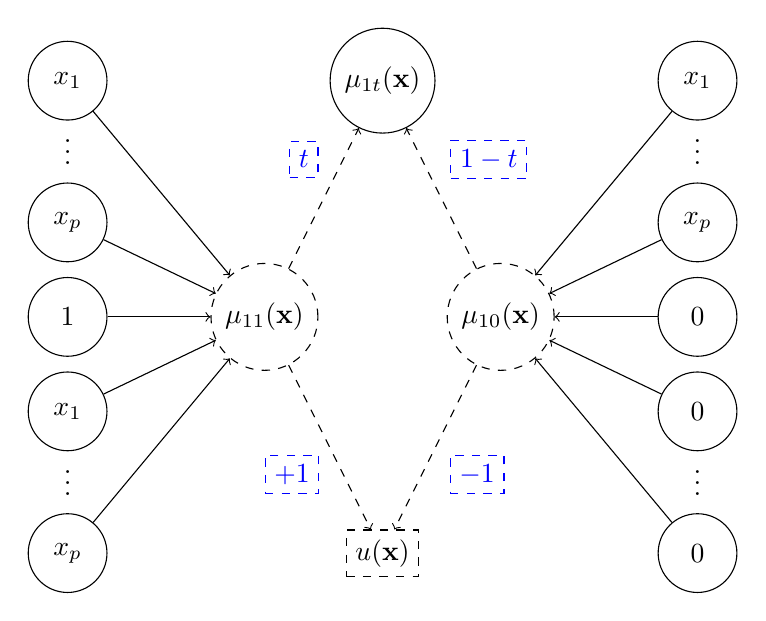
\begin{tikzpicture}
    
    
    \tikzset{dist/.style={path picture= {
    \begin{scope}[x=1pt,y=10pt]
      \draw plot[domain=-6:6] (\x,{1/(1 + exp(-\x))-0.5});
    \end{scope}
    }}}
    \tikzstyle{sigmoid}=[draw,fill=gray!20,circle,minimum size=30pt,inner sep=0pt,dist]
    
    
    % INPUT LAYER
    % T=1
    %\draw[red,thick,dashed] (0,2) circle (3mm);
    \node(x11) at (0,2) [circle,draw, minimum size=1cm] {$x_1$};
    \node at (0,1.2) {$\vdots$};
    %\draw[red,thick,dashed] (0,0) circle (3mm);
    \node(x1p) at (0,0.2) [circle,draw, minimum size=1cm] {$x_p$};
    %\draw[blue,thick,dashed] (0,-1) circle (3mm);
    \node(t1) at (0,-1) [circle,draw, minimum size=1cm] {$1$};
    %\draw[blue,thick,dashed] (0,-2) circle (3mm);
    \node(t1x11) at (0,-2.2) [circle,draw, minimum size=1cm] {$x_1$};
    \node at (0,-3) {$\vdots$};
    %\draw[blue,thick,dashed] (0,-4) circle (3mm);
    \node(t1x1p) at (0,-4) [circle,draw, minimum size=1cm] {$x_p$};
    
    % T=t
    %\draw[red,thick,dashed] (4,-1) circle (3mm);
    %\node(true_t) at (4,-1) {$t$};
    
    % T=0
    %\draw[red,thick,dashed] (8,2) circle (3mm);
    \node(x21) at (8,2) [circle,draw, minimum size=1cm] {$x_1$};
    \node at (8,1.2) {$\vdots$};
    %\draw[red,thick,dashed] (8,0) circle (3mm);
    \node(x2p) at (8,0.2) [circle,draw, minimum size=1cm] {$x_p$};
    %\draw[blue,thick,dashed] (8,-1) circle (3mm);
    \node(t0) at (8,-1) [circle,draw, minimum size=1cm] {$0$};
    %\draw[blue,thick,dashed] (8,-2) circle (3mm);
    \node(t0x21) at (8,-2.2) [circle,draw, minimum size=1cm] {$0$};
    \node at (8,-3) {$\vdots$};
    %\draw[blue,thick,dashed] (8,-4) circle (3mm);
    \node(t0x2p) at (8,-4) [circle,draw, minimum size=1cm] {$0$};
    
    % CONDITIONAL MEANS 
    %\node (p1)[sigmoid] at (2.5, -1) {};
    \node (p1)[] at (2.5, -1) [circle, draw, dashed] {$\mu_{11}(\x)$};
    %\node (p0)[sigmoid] at (5.5, -1) {};
    \node (p0)[] at (5.5, -1) [circle, draw, dashed] {$\mu_{10}(\x)$};
    
    % WEIGHTS
    \draw[->] (x11) -- (p1) ;% node [midway,above]% {$\beta_1$};
    \draw[->] (x1p) -- (p1) ;% node [midway,above] {$\beta_p$};
    \draw[->] (t1) -- (p1) ;% node [midway,above] {$\gamma$};
    \draw[->] (t1x11) -- (p1) ;% node [midway,above] {$\delta_1$};
    \draw[->] (t1x1p) -- (p1) ;% node [midway,above] {$\delta_p$};
    
    
    \draw[->] (x21) -- (p0) ;% node [midway,above] {$\beta_1$};
    \draw[->] (x2p) -- (p0) ;% node [midway,above] {$\beta_p$};
    \draw[->] (t0) -- (p0) ;% node [midway,above] {$\gamma$};
    \draw[->] (t0x21) -- (p0) ;% node [midway,above] {$\delta_1$};
    \draw[->] (t0x2p) -- (p0) ;% node [midway,above] {$\delta_p$};
    
    %OUTPUT
    %\draw[black,thick] (4,-4) circle (5mm);
    \node(uplift) at (4,-4) [rectangle, draw, dashed] {$u(\x)$};
    
    %\draw[black,thick] (4,2) circle (6mm);
    \node(mean) at (4,2) [circle, draw] {$\mu_{1t}(\x)$};
    
    %OUTPUT CONNEXIONS
    %\draw[->, dashed] (true_t) -- (mean);
    \draw[->, dashed] (p1) -- (mean); %node [midway,above] {$t$};
    \node at (3,1) [rectangle, dashed, blue, draw] {$t$};
    \draw[->, dashed] (p0) -- (mean); %node [midway,above] {$(1-t)$};
    \node at (5.35,1) [rectangle, dashed, blue, draw] {$1-t$};
    
    \draw[->, dashed] (p1) -- (uplift); %node [midway,above] {$+1$};
    \node at (2.85,-3) [rectangle, dashed, blue, draw] {$+1$};
    \draw[->, dashed] (p0) -- (uplift); %node [midway,above] {$-1$};
    \node at (5.2,-3) [rectangle, dashed, blue, draw] {$-1$};
    
    \end{tikzpicture}}
%    \caption{SMITE neural network architecture.}
%    \label{fig:nite}
%\end{figure}

    \caption{Siamese representation of the uplift interaction model.}
    \label{fig:siamese_network}
\end{figure}

The model can be written as follows:
\begin{align*}
  &\mu_{t_i}(\x_i, \theta_o, \boldsymbol{\theta}) = \mathrm{Pr} (Y_i = 1 \mid \mathbf{x}_i, t_i, \theta_o, \boldsymbol{\theta}) =
  \bigl( 1+ \mathrm{exp}\{-(\theta_o + \gamma t_i + \mathbf{x}_i^\top [\boldsymbol{\beta} + t_i \boldsymbol{\delta}] ) \} \bigr)^{-1},\\
  &u(\x_i) = \mu_1(\x_i) - \mu_0(\x_i) 
\end{align*}
where $\boldsymbol{\theta} = (\boldsymbol{\beta}, \gamma, \boldsymbol{\delta})$, denotes all model parameters except for the intercept $\theta_o$.


Some parts of the following subsections need work:

\begin{enumerate}
    \item The transformed outcome \textcolor{blue}{Almost done. Introduced the different transformed outcomes but need to elaborate a bit more on $Z$ and why MSE is not useful for binary $Y$.}
    \begin{enumerate}
        \item[a.1)] Regularized conditional means regression \textcolor{blue}{Almost done. We need to justify the exponential loss more clearly for SMITE TO.}
        \item[a.2)] The optimization algorithm \textcolor{red}{DONE. Elementary explanation of SGD and related references.}
    \end{enumerate} 
    \item Exploring other regularization functions \textcolor{blue}{This part needs work. We need Alejandro's input on the justification of SMITE IE and we can also discuss other types of losses.} \textcolor{red}{Check Alejandro's development of the IE likelihood.}
\end{enumerate}



\subsection{SMITE neural network}

\begin{figure}[H]
    \centering
    \scalebox{0.95}{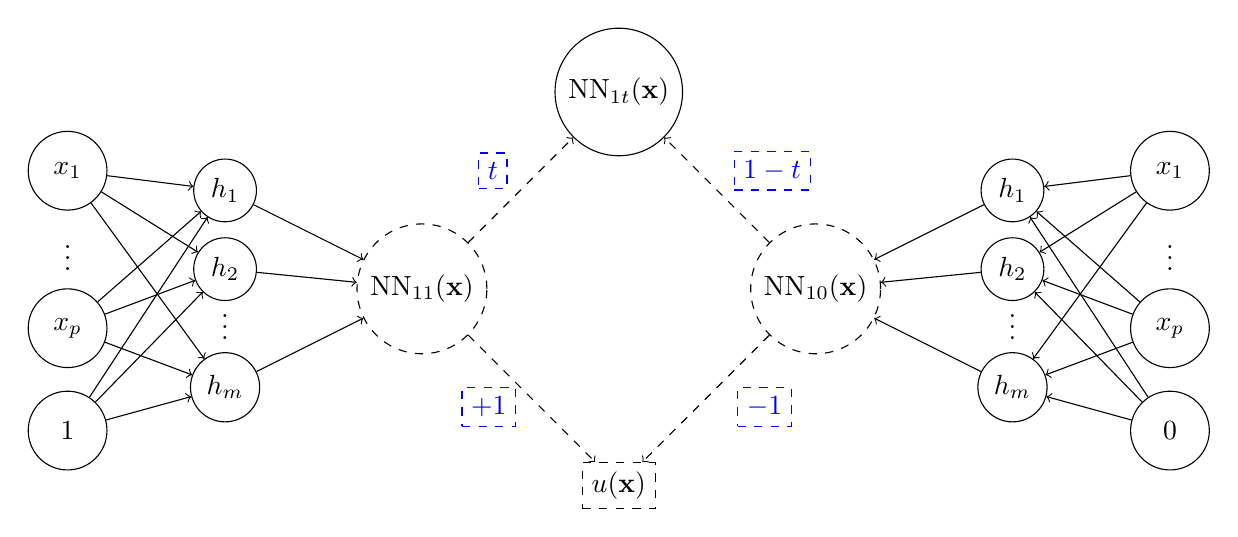
\begin{tikzpicture}
    
    
    \tikzset{dist/.style={path picture= {
    \begin{scope}[x=1pt,y=10pt]
      \draw plot[domain=-6:6] (\x,{1/(1 + exp(-\x))-0.5});
    \end{scope}
    }}}
    \tikzstyle{sigmoid}=[draw,fill=gray!20,circle,minimum size=20pt,inner sep=0pt,dist]
    
    
    % INPUT LAYER
    % T=1
    %\draw[red,thick,dashed] (-1,1) circle (3mm);
    \node(x11) at (-3,1) [circle, draw, minimum size=1cm] {$x_1$};
    \node at (-3,0) {$\vdots$};
    %\draw[red,thick,dashed] (-1,-1) circle (3mm);
    \node(x1p) at (-3,-1) [circle, draw, minimum size=1cm] {$x_p$};
    %\draw[blue,thick,dashed] (-1,-2) circle (3mm);
    \node(t1) at (-3,-2.3) [circle, draw, minimum size=1cm] {$1$};

    
    % T=0
    %\draw[red,thick,dashed] (9,1) circle (3mm);
    \node(x21) at (11,1) [circle, draw, minimum size=1cm] {$x_1$};
    \node at (11,0) {$\vdots$};
    %\draw[red,thick,dashed] (9,-1) circle (3mm);
    \node(x2p) at (11,-1) [circle, draw, minimum size=1cm] {$x_p$};
    %\draw[blue,thick,dashed] (9,-2) circle (3mm);
    \node(t0) at (11,-2.3) [circle, draw, minimum size=1cm] {$0$};
  
    % HIDDEN LAYER
    % T=1
    %\draw[black,thick,dashed] (1,0.75) circle (3mm);
    \node(h11) at (-1,0.75) [circle, draw] {$h_1$};
    %\draw[black,thick,dashed] (1,0) circle (3mm);
    \node(h12) at (-1,-0.25) [circle, draw] {$h_2$};
    \node at (-1,-0.875) {$\vdots$};
    %\draw[black,thick,dashed] (1,-1.75) circle (3mm);
    \node(h1m) at (-1,-1.75) [circle, draw] {$h_m$};
     % T=0
    %\draw[black,thick,dashed] (7,0.75) circle (3mm);
    \node(h21) at (9,0.75) [circle, draw] {$h_1$};
    %\draw[black,thick,dashed] (7,0) circle (3mm);
    \node(h22) at (9,-0.25) [circle, draw] {$h_2$};
    \node at (9,-0.875) {$\vdots$};
    %\draw[black,thick,dashed] (7,-1.75) circle (3mm);
    \node(h2m) at (9,-1.75) [circle, draw] {$h_m$};
    
    % CENTER OF THE FIGURE
    % T=t
    %\draw[red,thick,dashed] (4,-0.5) circle (3mm);
    %\node(true_t) at (4,-0.5) {$t$};
    % CONDITIONAL MEANS 
    %\draw[black,thick,dashed]  (2.5, -0.5) circle (7mm);
    \node (p1)[] at (1.5, -0.5) [circle, draw, dashed] {$\mathrm{NN}_{11}(\x)$};
    %\node (p1)[sigmoid] at (2.5, -0.5) {};
    %\node (p0)[sigmoid] at (5.5, -0.5) {};
    %\draw[black,thick,dashed]  (5.5, -0.5) circle (7mm);
    \node (p0)[] at (6.5, -0.5) [circle, draw, dashed] {$\mathrm{NN}_{10}(\x)$};
    
    % WEIGHTS
    %1st layer T=1
    \draw[->] (x11) -- (h11) node [midway,above] {};
    \draw[->] (x1p) -- (h11) node [midway,above] {};
    \draw[->] (t1) -- (h11) node [midway,above] {};
    
    \draw[->] (x11) -- (h12) node [midway,above] {};
    \draw[->] (x1p) -- (h12) node [midway,above] {};
    \draw[->] (t1) -- (h12) node [midway,above] {};
    
    \draw[->] (x11) -- (h1m) node [midway,above] {};
    \draw[->] (x1p) -- (h1m) node [midway,above] {};
    \draw[->] (t1) -- (h1m) node [midway,above] {};
    
    %1st layer T=0
    \draw[->] (x21) -- (h21) node [midway,above] {};
    \draw[->] (x2p) -- (h21) node [midway,above] {};
    \draw[->] (t0) -- (h21) node [midway,above] {};
    
    \draw[->] (x21) -- (h22) node [midway,above] {};
    \draw[->] (x2p) -- (h22) node [midway,above] {};
    \draw[->] (t0) -- (h22) node [midway,above] {};
    
    \draw[->] (x21) -- (h2m) node [midway,above] {};
    \draw[->] (x2p) -- (h2m) node [midway,above] {};
    \draw[->] (t0) -- (h2m) node [midway,above] {};
    
    %2nd layer
    \draw[->] (h11) -- (p1) node [midway,above] {};
    \draw[->] (h12) -- (p1) node [midway,below] {};
    \draw[->] (h1m) -- (p1) node [midway,below] {};
    
    \draw[->] (h21) -- (p0) node [midway,above] {};
    \draw[->] (h22) -- (p0) node [midway,below] {};
    \draw[->] (h2m) -- (p0) node [midway,below] {};
    
    
    %OUTPUT
    %\draw[black,thick] (4,-3) circle (6mm);
    \node(uplift) at (4,-3) [rectangle, draw, dashed] {$u(\x)$};
    
    %\draw[black,thick] (4,2) circle (7mm);
    \node(mean) at (4,2) [circle, draw] {$\mathrm{NN}_{1t}(\x)$};
    
    %OUTPUT CONNEXIONS
     %\draw[->, dashed] (true_t) -- (mean);
    \draw[->, dashed] (p1) -- (mean); %node [midway,above] {$t$};
    \node at (2.4,1) [rectangle, draw, blue, dashed] {$t$};
    \draw[->, dashed] (p0) -- (mean); %node [midway,above] {$(1-t)$};
    \node at (5.95,1) [rectangle, draw, blue, dashed] {$1-t$};
    
    \draw[->, dashed] (p1) -- (uplift); %node [midway,above] {$+1$};
    \node at (2.35,-2) [rectangle, draw, blue, dashed] {$+1$};
    \draw[->, dashed] (p0) -- (uplift); %node [midway,above] {$-1$};
    \node at (5.85,-2) [rectangle, draw, blue, dashed] {$-1$};
    
    
    \end{tikzpicture}}
    \caption{A twin neural model for uplift. The inputs contain the covariates vector $\x$ and, for the left sub-component, the treatment variable fixed to $1$. The treatment variable is fixed to $0$ for the right sub-component. The sub-components output the predicted conditional means for treated ($\mathrm{NN}_{11}(\x)$) and for control ($\mathrm{NN}_{10}(\x)$). The difference gives direct prediction of $u(\x)$. At the same time, the predicted conditional mean $\mathrm{NN}_{1t}(\x)$ is based on the actual received treatment for each individual $t \in \{0,1\}$, i.e., $\mathrm{NN}_{1t}(\x) = t \mathrm{NN}_{11}(\x) + (1-t) \mathrm{NN}_{10}(\x)$.}
    \label{fig:nite}
\end{figure}


In this section, we generalize to the neural networks version of SMITE. \textcolor{blue}{We will need Alejandro's input on what is next. Based on discussions with Vahid, this section will be arranged as follows:}

\begin{enumerate}
    \item Universal approximation theorems \textcolor{red}{DONE}
    \item Low-rank approximation \textcolor{red}{DONE} 
    \item Low-rank SMITE \textcolor{blue}{TO DO. This part can be related to model selection ! Needs more discussions.}
\end{enumerate}

The first two subsections are brief literature reviews on the subject. The last one needs a clear connection with SMITE. Here are Alejandro's comments on the subject: 

\textit{We do not necessarily study low rank approximations of the matrix of weights. For this you will need indeed to get bounds on the distance between the estimated function and the approximation function. In Statistics, usually we just measure the statistical difference between two models (and not the distance between the two models). So instead of thinking of a reduced approximation of the weight matrix, we might just think of a model with a lower-rank matrix of weights. This in general will lead to a non-parametric estimator with lower variance and hopefully, only slightly increased bias. In this setup, methods to measure the statistical difference between the full model and the reduced model should be applied for each dataset. This is in contrast to the general approximation theory, where bounds on the approximation error over all possible datasets need to be found.}

\subsection{Evaluating uplift models}

This section introduces the Qini measures. I believe we should also define the ITE related metrics such as $\mu$-risk, $\tau$-risk and $v$ that stands for {\it value} which is somehow related to the gain chart sometimes used in marketing. \textcolor{blue}{TO DO} 

\textcolor{red}{On Kendall and Qini coefficients (and associated curves), we need to discuss and develop some geometrical intuition behind these statistics. We can present these with a different way of thinking.}

\subsection{Experiments}

We already have results but I think we need to discuss which experiments we want to run in order to be able to improve this part of the work. \textcolor{blue}{TO DO}


\section{Coding/Experiments}

All codes are ready and clean. We only need to run the necessary experiments and list the Figures we want to show in the paper. \textcolor{blue}{TO DO}

\section{Data}

The problem with public datasets used in ITE literature is that they are observational. We need to decide on which datasets we work. I think that we could also use the dataset used in the Qini-based paper to be able to compare the results without re-running all the experiments. \textcolor{blue}{TO DO}


\end{document}